\documentclass[12pt,a4paper,twoside]{article}

\usepackage{fancyhdr}
\usepackage{lastpage}
\usepackage{geometry} 
\usepackage{amsmath}
\usepackage{amssymb} 
\usepackage{graphicx}
\usepackage{wrapfig}
\usepackage{color}
\usepackage{fancybox}
\usepackage[T1]{fontenc}
% \usepackage{hangcaption}
\usepackage{listings}
\usepackage[utf8]{inputenc}
\usepackage[francais]{babel}

% Indent with space between paragraphs rather than indentation
% https://tex.stackexchange.com/questions/42/
\usepackage{parskip}

\usepackage{enumitem}

\geometry{
	margin=2.5cm,
	includeheadfoot,
}

\title{Title}
\author{Nom Prénom}
\date{\today}

\begin{document}

\lstset{numbers=left, tabsize=3, frame=single, numberstyle=\ttfamily,
		basicstyle=\footnotesize} 
\thispagestyle{empty}

\section{Le CEA}
Acteur majeur de la recherche, du développement et de l'innovation, le
Commissariat à l'énergie atomique et aux énergies alternatives intervient dans
le cadre de quatre missions :

\begin{itemize}[label=\textbullet]
	\item	la défense et la sécurité ;
	\item	l'énergie nucléaire (fission et fusion) ;
	\item	la recherche technologique pour l'industrie ;
	\item	la recherche fondamentale (sciences de la matière et sciences
		de la vie).
\end{itemize}

S'appuyant sur une capacité d'expertise reconnue, le CEA participe à la mise en
place de projets de collaboration avec de nombreux partenaires académiques et
industriels.

Le CEA est implanté sur 10 centres répartis dans toute la France. Il développe
de nombreux partenariats avec les autres organismes de recherche, les
collectivités locales et les universités. A ce titre, le CEA est partie prenante
des alliances nationales coordonnant la recherche française dans les domaines de
l'énergie (ANCRE), des sciences de la vie et de la santé (AVIESAN), des sciences
et technologies du numérique (ALLISTENE), des sciences de l'environnement
(ALIEnv) et des sciences humaines et sociales (ATHENA).

Reconnu comme un expert dans ses domaines de compétence, le CEA est pleinement
inséré dans l'espace européen de la recherche et exerce une présence croissante
au niveau international.

Le CEA compte 16 110 techniciens, ingénieurs, chercheurs et collaborateurs pour
un budget de 4,4 milliards d'euros (chiffres publiés fin 2014).

\begin{figure}[b]
	\centering
	\makebox[\textwidth]{
		\raisebox{-80pt}[0pt][10pt]{
			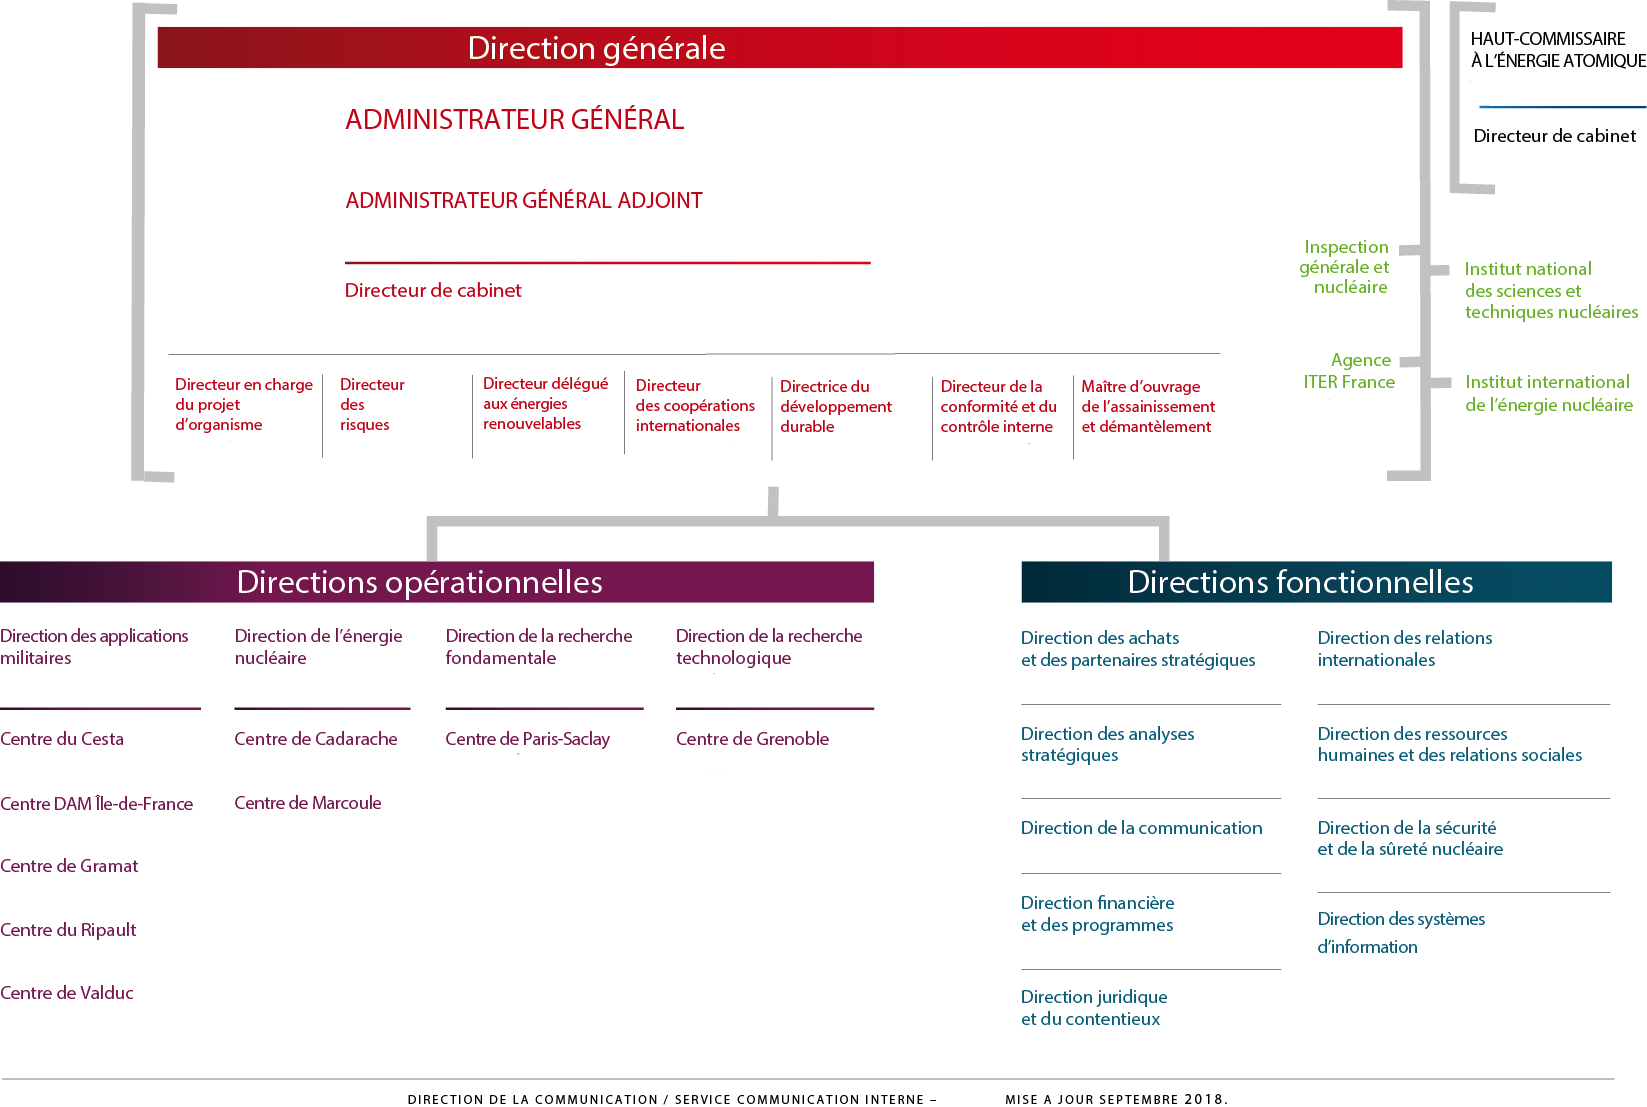
\includegraphics[width=0.8\textwidth]{ressources/diagrammes/organigramme_cea.png}
		}
	}
\end{figure}

\newpage

\section{La direction des applications militaires}

\subsection*{Une direction au service de la dissuasion}
La Direction des applications militaires (DAM) du CEA, a pour mission
de concevoir, fabriquer, maintenir en condition opérationnelle, puis démanteler
les têtes nucléaires qui équipent les forces nucléaires aéroportée et océanique
françaises.

La DAM est chargée de la conception et de la réalisation des réacteurs et de
c\oe urs nucléaires équipant les bâtiments de la Marine nationale, sous-marins
et porte-avions. Elle apporte son soutien à la Marine nationale pour le suivi en
service et le maintien en condition opérationnelle de ces réacteurs.

La DAM est également responsable de l'approvisionnement des matières nucléaires
straté\-giques pour les besoins de la dissuasion.

Dans un monde en profonde mutation, la DAM contribue aussi à la sécurité
nationale et
\begin{wrapfigure}[12]{r}{10cm}
	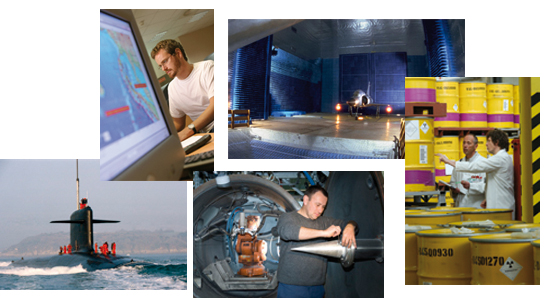
\includegraphics[width=10cm]{ressources/images/dam/5_thumbnails.jpg}
\end{wrapfigure}
internationale à travers l'appui technique qu'elle apporte aux autorités, pour
les questions de lutte contre la prolifération nucléaire et le terrorisme et de
désarmement.

Depuis le transfert du centre de Gramat en 2010 de la Direction générale de
l'armement au CEA, la DAM apporte son expertise à la Défense dans le domaine de
l'armement conventionnel.

\subsection*{Une direction ouverte à la recherche}
Le partage national et international des connaissances (lorsqu'il est possible),
la confrontation à l'évaluation scientifique extérieure, l'intégration à des
réseaux de compétences constituent des gages de crédibilité scientifique.

Les équipes de la DAM réalisent chaque année environ 2000 publications et
communications scientifiques. Cette ouverture de la DAM passe également par la
mise à la disposition de la communauté des chercheurs de ses moyens
expérimentaux et par la contribution de ses équipes à d'autres programmes de
recherche.

\subsection*{Une direction actrice de la politique industrielle française}
La DAM partage très largement son activité avec l'industrie française : c'est
ainsi que le montant des achats, auprès de celle-ci, représente plus des deux
tiers de son budget ; le dernier tiers se répartit entre les salaires des
personnels (un cinquième) et les taxes.

La politique industrielle de la DAM est originale à plus d'un titre :

\begin{itemize}[label=\textbullet]
	\item
		d'abord parce que la DAM conserve la maîtrise d'\oe uvre
		d'ensemble de la grande majorité des systèmes dont elle a la
		responsabilité : elle veille ainsi au juste équilibre entre les
		grands groupes industriels de la Défense et les PME souvent
		innovantes, en contractualisant directement avec ces dernières,
		leur permettant ainsi de recevoir la juste rémunération de leur
		production ;
	\item	
		ensuite, parce que la répartition de son budget est sous-tendue
		par une répartition des travaux : la DAM conduit la recherche
		dans ses laboratoires grâce à son personnel de haut niveau
		scientifique et technologique. Une fois la définition d'un
		produit acquise, la DAM transfère la définition et les procédés
		vers les industriels qui en réalisent le développement, puis la
		production.
\end{itemize}

La DAM a également pour objectif que ses centres participent à la vie économique
locale par leur implication dans les pôles de compétitivité. Hors de son propre
champ d'utilisation, elle valorise ses recherches par le transfert de
technologies vers l'industrie et le dépôt de nombreux brevets.

\subsection*{Le format}
La DAM comprend cinq centres aux missions homogènes, dont les activités se
répartissent entre la recherche de base, le développement et la fabrication :
\begin{figure}[!ht]
	\begin{minipage}{0.6\linewidth}
		\begin{itemize}[label=\textbullet]
			\item
				{\bf DAM Ile-de-France (DIF)}, à Bruyères-le-Châtel, où sont
				menés les travaux de physique des armes, les activités de
				simulation numérique et de lutte contre la prolifération
				nucléaire ; DIF est aussi le centre responsable de l'ingénierie
				à la DAM ; enfin, au centre DIF est rattachée l'INBS-Propulsion
				Nucléaire du centre CEA/Cadarache, en région Provence Alpes-Côte
				d'Azur, où sont implantées les installations d'essais à terre et
				une partie des fabrications de la propulsion nucléaire ;
		\end{itemize}
	\end{minipage}
	\begin{minipage}{0.4\linewidth}
		\centering
		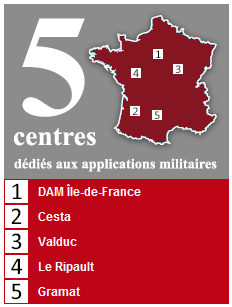
\includegraphics[width=0.7\textwidth]{ressources/images/dam/5_centres.png}
	\end{minipage}
\end{figure}

\begin{itemize}[label=\textbullet]
	\item
		{\bf Le Cesta}, en Aquitaine, consacré à l'architecture des armes, aux
		tests de tenue à l'environnement. Il met en oeuvre le Laser Mégajoule,
		équipement majeur de la Simulation ;
	\item
		{\bf Valduc}, en Bourgogne, dédié aux matériaux nucléaires et à
		l'installation expérimentale Epure du programme Simulation ;
	\item
		{\bf Le Ripault}, en région Centre, dédié aux matériaux non nucléaires
		(explosifs chimiques...) ;
	\item
		{\bf Gramat}, (ex-DGA) en Midi-Pyrénées, qui conduit au profit de la
		Défense des activités en vulnérabilité des systèmes et efficacité des
		armements.
\end{itemize}

\begin{figure}[b]
	\begin{center}
		\makebox[\textwidth]{
			\raisebox{70pt}[0pt][0pt]{
				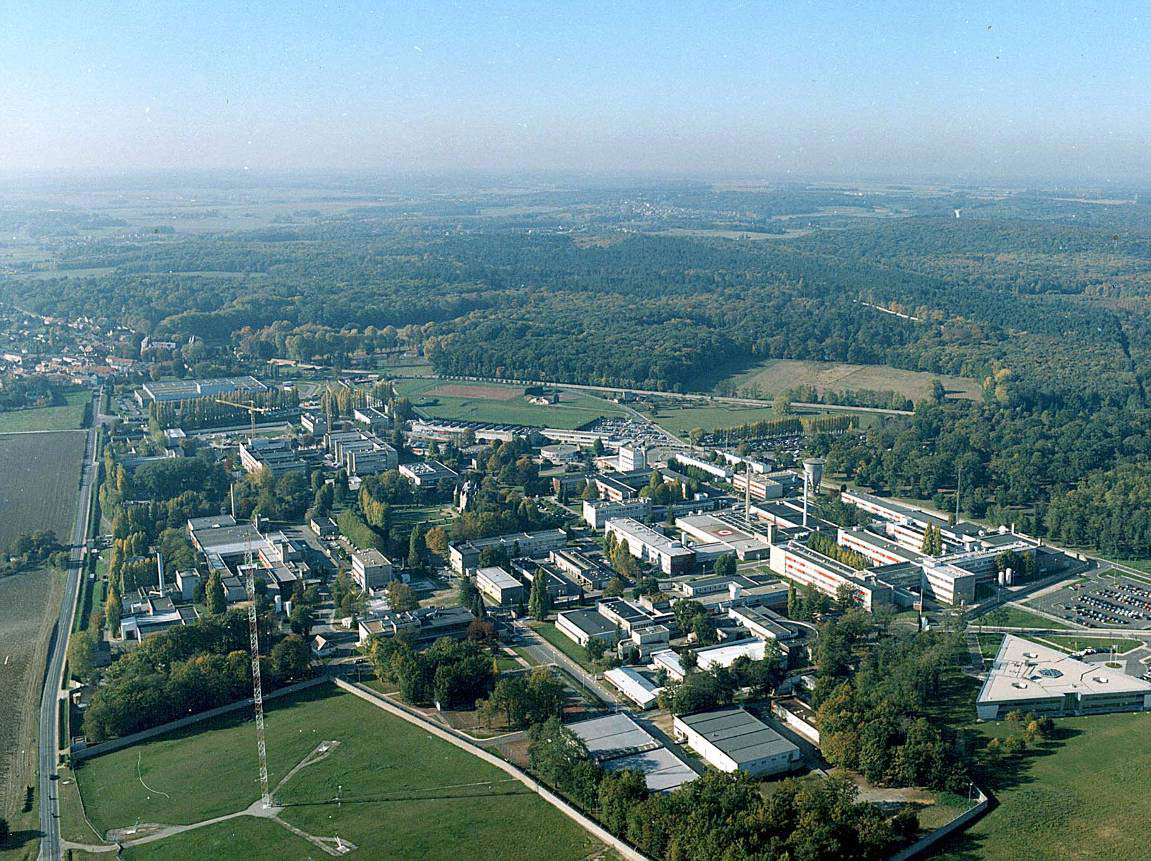
\includegraphics[scale=0.4]{ressources/images/dam/vue_aerienne.png}
			}
		}
		\caption{Centre DAM Ile-de-France}
	\end{center}
\end{figure}

\newpage

\end{document}
